\documentclass[11pt,a4paper]{scrartcl}

\usepackage{xcolor}
\usepackage{float}
\usepackage{subfig}
\usepackage[T1]{fontenc}
\usepackage{graphicx}
\usepackage[automark]{scrlayer-scrpage}
\usepackage[hidelinks]{hyperref}
\usepackage{listings}
\usepackage{enumitem}
\usepackage[left=2cm, right=2cm, top=2cm, bottom=2cm]{geometry}
\graphicspath{{./img/}}
\setlength{\parindent}{0em} 

\hypersetup{
  colorlinks=true,
  linkcolor=black, %!70!black,
  urlcolor=blue!70!black
}

\let\oldsection\section
\renewcommand\section{\clearpage\oldsection}

\makeindex

\pagestyle{scrheadings}
\clearscrheadfoot
\ofoot[\pagemark]{\pagemark}
\ihead[]{\headmark}
\setheadsepline[\textwidth]{0.5pt}

\title{Final Report}
\author{Marc Berli, Simon Stucki, ...}
\date{\today{}, Zürich}

\begin{document}

\begin{titlepage}
  \centering
  {\scshape\LARGE PSIT4 \par}
  \vspace{1cm}
  {\scshape ZHAW - School of Engineering\par}
  \vspace{1cm}
  {\scshape\Large Darwin\par}
  \vspace{1.5cm}
  {\huge\bfseries Software Guidebook\par}
  \vspace{2cm}
  von
  \vspace{1em}
  \Large\itshape \\ Raphael Mailänder, Marc Berli, Ferenc Kuntić \\ Michael Schaufelberger, Filip Kašiković und Simon Stucki\par
  \vfill
  \textbf{Team}\par
  IT17ta\_ZH\par
  \vspace{2em}
  \textbf{Status}\par
  In Progress

  \vfill

  {\large \today \textbf{ --} Zürich\par}
\end{titlepage}

\tableofcontents

\newpage

\section{Kontext}
% Dieser erste Teil des Dokuments beschreibt grob die Idee des Produktes und das Umfeld des
% Produktes. Dieses Kapitel muss nicht lang sein (halbe bis max. 2 Seiten) und sollte folgende
% Fragen beantworten:
% • Um was geht es bei der Software, dem Produkt, dem System?
% • Was wird produziert?
% • Wie passt es ins bestehende Umfeld?
% • Wer verwendet die Software? (Aktoren, Anwender, Rollen, ...)
% Dieses Kapitel muss in jedem Software-Guidebook enthalten sein.

Die Idee des Projekts ist es, ein Spiel zu entwickeln, welches sich nicht durch klassische Echtzeiteingaben,
sondern durch Code steuern lässt.
Der Spieler schreibt dazu ein Skript, welches in einer Schleife ausgeführt wird.
Er kann mittels des Skripts beispielsweise den aktuellen Spielstand auslesen, Berechnungen anstellen und zum Schluss eine Liste von vordefinierten Aktionen durchführen.

Das Spiel selbst ist in seiner Grundform ein Multiplayer Survival Game.
Es treten mehrere Spieler gegeneinander an.
Ziel des Spiels ist es, der einzige Überlebende zu sein.
Dazu müssen Einheiten der Spieler beispielsweise Essen aufsammeln, um nicht zu verhungern, PowerUps brauchen, um beispielsweise ihre Verteidigung zu verbessern, oder können gegnerische Einheiten angreifen.
Dieses simple Spielprinzip ist für Spieler einfach zu verstehen oder bereits bekannt.
Die Steuerung durch den Code erlaubt uns, den Schwerpunkt des Gameplays stärker auf die Vorausplanung und langfristigen Strategien zu legen und reaktives Gameplay in den Hintergrund zu stellen.

\begin{figure}[h]
  \centering
  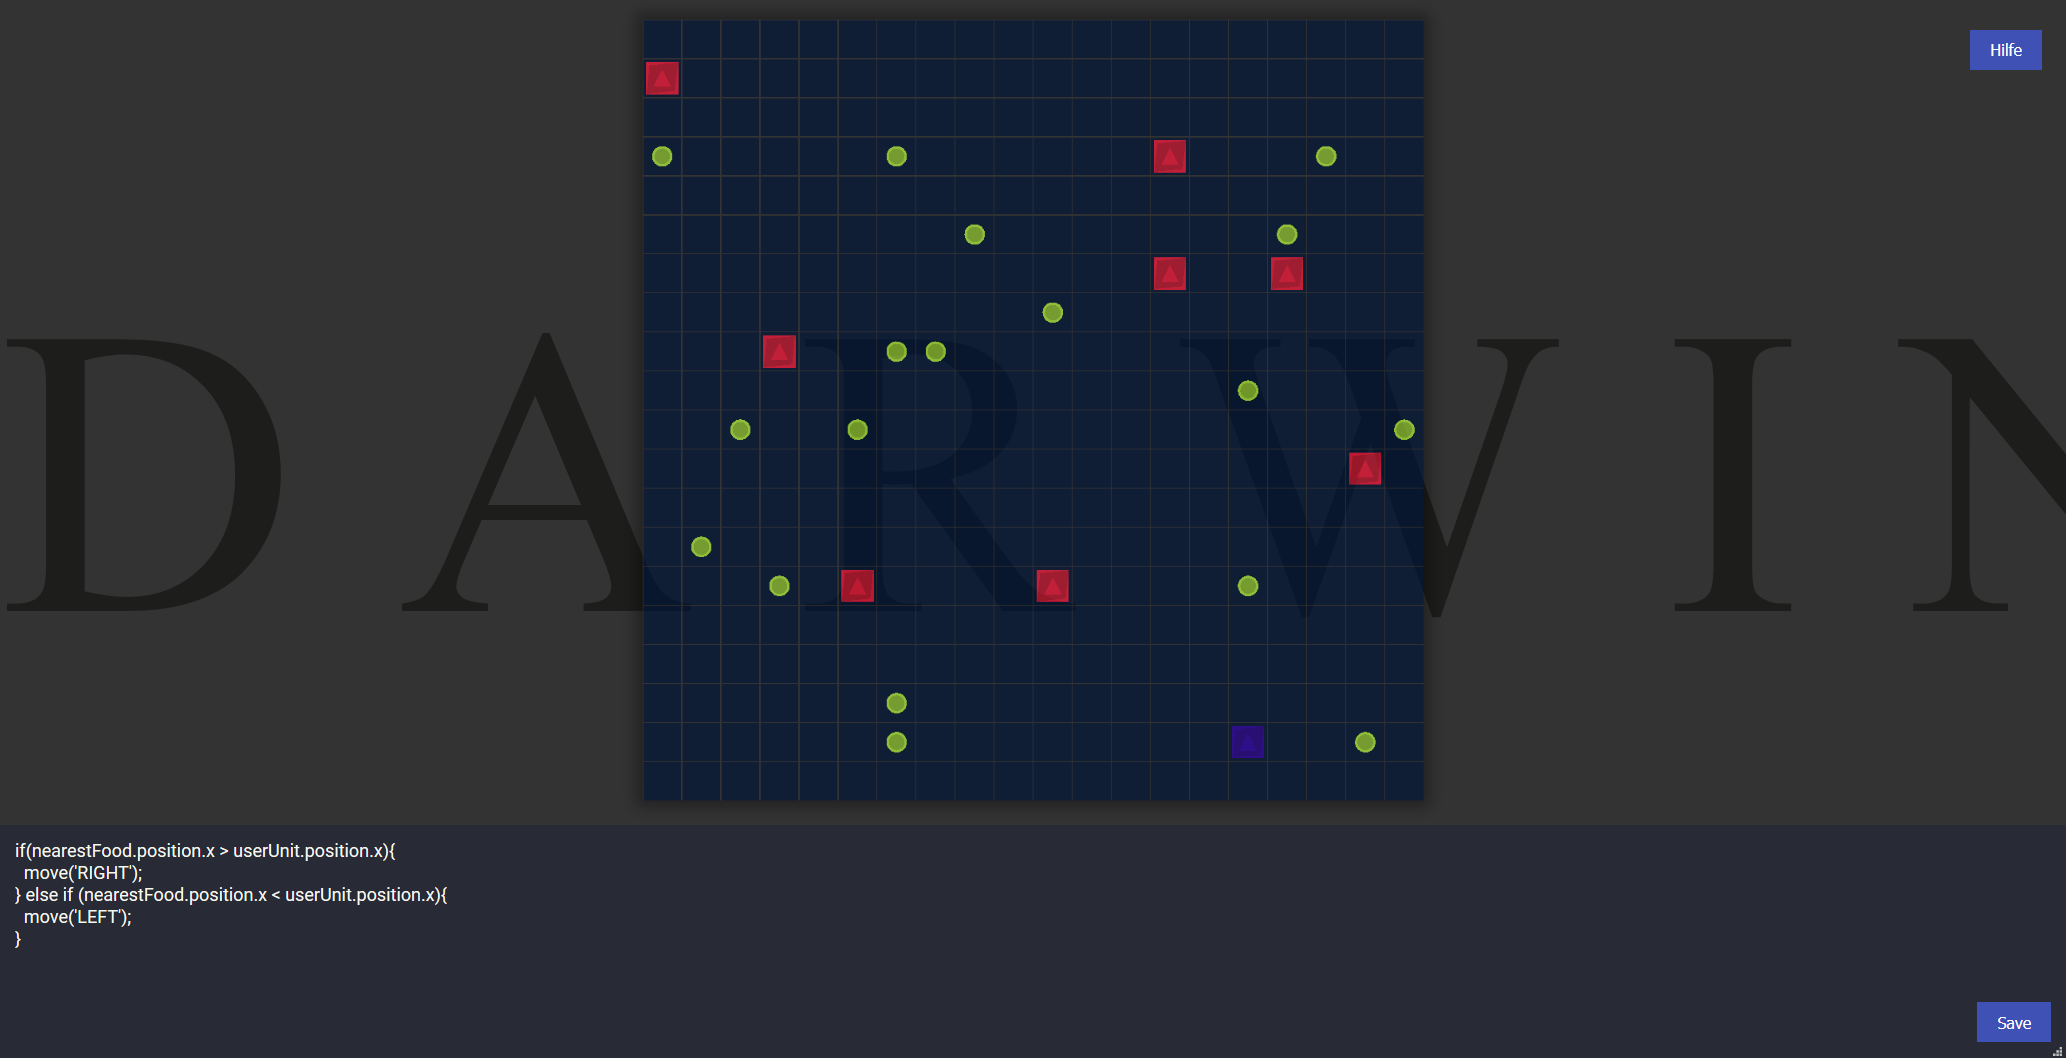
\includegraphics[width=0.95\textwidth]{darwin-gameplay}
  \caption{Darwin Gameplay}
\end{figure}

Da in unserem Team niemand Erfahrung mit Grafikdesign hat, möchten wird das Gametheme möglichst einfach halten.
Alle Objekte im Spiel werden als geometrische Form dargestellt, welche allenfalls kleine Modifikationen (zum Beispiel ein rotes Dreieck mit einem Punkt in der Mitte) aufweisen.
So wird die Darstellung des Spiels einfacher, bleibt aber trotzdem noch ansprechend.

Das Spiel wird als Webapplikation umgesetzt.
Spieler können sich gegenseitig herausforden und ein Match starten.
Während des Spielverlaufs können sie ihr Skript aktualisieren und visuell verfolgen, wie das Spielfeld aktuell aussieht. Zuschauer sehen nur den aktuellen Spielstand.

Für die Entwicklung unseres Spieles wird Github und Azure DevOps verwendet,
währenddessen als Hauptprogrammiersprache, im Backend sowie im Frontend, TypeScript zum Einsatz kommt.

Das Spiel richtet sich auf leidenschaftliche und engagierte Software Entwickler aus, die ihr Können unter Beweis stellen und sich mit Kollegen messen möchten.

\subsection{User Roles}
In diesem Abschnitt werden die User Roles genauer beschrieben. Sie sind die Hauptbenutzer des Spiels.
\subsubsection{Player}
Der Player ist der Hauptbenutzer des Spiels. Er verwendet die Software häufig. Sein Hauptziel ist es, mittels Code seine Units zu steuern, um möglichst lange im Spiel zu überleben. Da der Code die einzige Möglichkeit ist, das Spiel zu steuern möchte er den Code möglichst bequem (mittels Syntax-Highlighting) eingeben.
\subsubsection{Spectator}
Der Spectator ist ein Zuschauer des Spiels. Er ist wie der Player mit den Regeln des Spiels vertraut, möchte aber nur eine Arena sehen und nicht selbst spielen.
\subsubsection{User}
Der User ist Player und Spectator zusammengefasst. Also alle Personen, welche das Spiel in irgendeiner Form verwenden.
\subsubsection{Unit}
Die Unit ist eine logische Rolle. Ihr Ziel ist zu Überleben, kann das aber nicht selbst beeinflussen, da sie vom Player gesteuert wird. Diese Rolle vereinfacht das Schreiben von User Stories für den Spielablauf und die Ausbalanciertheit des Spiels.

\section{Ziele und Hauptfunktionen}
%• Ist allen Teilnehmern klar, was das System, die Software macht?
%• Welche Funktionen sind essentiell für den Erfolg des Produkts
%• Wann ist es ein Erfolg? Welche Ziele müssen erreicht werden? (quantitative technische,
%wirtschaftliche oder organisatorische Ziele)
% Spiel beschreiben und das so kleinwenig das technische ansprechen

Die essenziellen Komponenten des Spieles sind einerseits das Backend, das es erlaubt den vom Spieler verfassten Code auszuführen und andererseits das Frontend, welches es dem Benutzer ersichtlich macht, was für Auswirkungen sein Code hat. Zusätzlich dazu braucht es ein faires Game Balancing, durch das es möglich ist mit verschiedensten Strategien zu gewinnen:

\begin{itemize}
  \item Zuschauer können einem Match beitreten, ohne dass sie Einheiten kontrollieren können. \href{https://dev.azure.com/schaumic/darwin/_workitems/edit/43/}{\#43 Spectators}
  \item Die Spieler und Zuschauer können das Match visuell mitverfolgen. \href{https://dev.azure.com/schaumic/darwin/_workitems/edit/21/}{\#21 Arena Update}
  \item Die Spieler können das Spiel mittels Code steuern. \href{https://dev.azure.com/schaumic/darwin/_workitems/edit/20/}{\#20 Move Command}
  \item Der Spieler kann die Spielregeln sowie eine Liste aller verfügbaren Aktionen der Einheiten abrufen. \href{https://dev.azure.com/schaumic/darwin/_workitems/edit/22/}{\#22 Help}
\end{itemize}

Sofern diese vier Punkte erfolgreich umgesetzt werden können, gilt der technische Durchstich als erfolgreich. Alle weiteren Entwicklungen sind Verbesserungen dieser Ziele und dienen der Attraktivitätssteigerung des Spiels.

Des Weiteren soll das Spiel kostenlos als Webapplikation zur Verfügung stehen. Das Spiel könnte später mittels Werbung finanziert werden.

\section{Qualitätsattribute}
%• Welche Qualitätsattribute soll die Software/das System erfüllen?
%• Sind die Qualitatsatribute SMART (specific, measurable, achievable, relevant, timely)?
%• Gibt es Attribute, die üblicherweise als gegeben betrachtet werden explizit ausgenommen sind?
%• Sind alle Attribute und Anforderungen realistisch?

Qualitätsattribute:
\begin{itemize}

  \item Performance - Das Spiel soll den eingegeben Code innerhalb wenigen Sekunden kompilieren und ausführen.
  \item Verfügbarkeit - Der Server soll möglichst 24 Stunden am Tag laufen, da bei einem Unterbruch die aktuellen Matches beeinträchtigen oder sogar beendet werden würden.
  Ein fehlerhaftes Skript eines Spielers darf keine anderen Spieler beeinträchtigen.
  \item Security - Eine Prüfung auf schädlichen Code sowie Standard gegen 'Javascript Injection' müssen geprüft und ggf. implementiert werden.
  \item Erweiterbarkeit - Die Software muss modular aufgebaut sein, um einzelne Funktionen und Features einfach zu erweitern.
  \item Benutzerfreundlichkeit - Das Userinterface soll es ermöglichen, die gesuchten Infos möglichst schnell, unmittelbar und bequem bereitzustellen und es muss dem User erlauben, dass er sich auf der Seite bewegen kann, ohne auf Probleme zu stossen.
  \item Browserkompatibilität - Für die Browser Chrome und Firefox muss das Spiel konsistent funktionieren.
  \item Sprache - Das Spiel ist in der Deutschen Sprache verfügbar.
\end{itemize}

\section{Bekannte Beschränkungen}
%• Zeit
%• Budget und Ressourcen
%• Technologievorgaben
%• Ziel-Plattform
%• Standardprotoklle
%• Grösse des Entwicklungsteams
%• Kompetenzenprofil des Entwicklungsteams
%• lokale Standards

Bei unserer Software-Entwicklung werden die Prozesse von Story Beschreibung, Entwicklung, Testing und Code-Review befolgt und eingehalten.

Unsere Software ist unabhängig des Entwicklungsprozesses folgenden Beschränkungen ausgesetzt.
\begin{itemize}
  \item Zeit: Die Zeitdauer des Projekts ist eingeschränkt und beläuft sich auf 6 Sprints à je zwei Wochen.
  \item Budget und Ressourcen: Das Projekt ist ein Schulprojekt und ist deshalb grundsätzlich auf die Anzahl ECTS-Credits pro Entwickler beschränkt. In Stunden sind das ungefähr 100 bis 120 pro Entwickler, was Total 600 - 720 Stunden ergibt.
  \item Technologien: Wir verwenden die Technologien React und Node.js mit TypeScript. Grundsätzlich enthält das Projekt aber keine Technologievorgaben. Zurzeit verwenden wir zudem folgende Cloud Services für die Entwicklung, welche einzuhalten sind.
        \begin{itemize}
          \item Github - Als Git-Repository und für PR Reviews
          \item Azure DevOps - Als Projektplanungstool sowie für CI/CD Pipelines
        \end{itemize}
  \item Grösse des Entwicklungsteams: Das Team besteht aus einem Product Owner, einem Scrum Master und 4 weiteren Entwicklern.
  \item Kompetenzenprofil: Die Entwickler sind aktuell Teilzeitstudenten an der ZHAW und befinden sich im drittletzten Semester des Bachelorstudiengangs Informatik. Dadurch sind sie mit den Grundlagen der Objektorientierten Programmierung sowie mit den Technologien, die im Webbereich zum Einsatz kommen, vertraut. Desweiteren haben einige Entwickler bereits mehrjährige Berufserfahrung mit den Technologien React, TypeScript und Node JS.
  \item Datenpersistierung wird vernachlässigt, da es für die Zeitdauer dieses Projekts Out-of-Scope ist.
\end{itemize}

\section{Verwendete Prinzipien}
Um die Qualität der Software bei der Entwicklung unseres Spieles sicherzustellen, haben wir uns auf folgende Prinzipien geeinigt.

\subsection{Generelles}
\begin{itemize}
  \item Anstatt direkt in den Master-Branch zu pushen, wird für jede Änderung ein Branch erstellt, welcher mittels eines Pull-Request in den Master-Branch gemerged wird.
        So können wir sicherstellen, dass der Code und die in Entwicklung begriffenen Änderungen den Vorstellungen des Teams entsprechen.
  \item Bevor ein Pull-Request gemerged wird, prüfen wir mittels einer automatisierten Build-Pipeline, ob die Unit-Tests erfolgreich laufen.
  \item Fehlerbehandlungen werden grundsätzlich mittels 'Bug Stories' abgearbeitet, ausser sie können in einem PR Review o.ä. direkt erkannt und behoben werden.
  \item Wir kommunizieren offen und ehrlich miteinander.
\end{itemize}

\subsection{Coding}
\begin{itemize}
  \item Hohe Kohäsion und minimale Kopplung ist wichtiger Bestandteil, um die Komplexität unseres Spieles zu minimieren und die Fehlerbehebung zu vereinfachen.
  \item Es wird grundsätzlich Funktionale Programmierung mit dem Immutability Prinzip eingesetzt.
  \item Coding Guidelines werden für unsere Entwicklung eingesetzt und mittels Eslint und TSlint sowie Pull-Request Reviews überprüft. So können Syntax und Code-Styling eingehalten werden.
\end{itemize}

\subsection{DoD}
Wir halten uns bei unserem Entwicklungsprozess an die folgende Definition of Done:
\begin{itemize}
  \item Alle Akzeptanzkriterien werden erfüllt.
  \item Der Code ist fertiggestellt und im Versionierungssystem eingespielt.
  \item Dokumentation aktualisiert.
  \item Es wurde ein Code Review durchgeführt oder der Code wurde im Pair Programming erarbeitet.
  \item Coding Guidelines und Standards wurden eingehalten.
  \item Unittests und Integrationtests wurden erfolgreich durchgeführt.
  \item Es sind keine kritischen Bugs offen.
\end{itemize}

\subsection{Testing}
Das Testen der Applikation erfolgt in drei Schritten:

\subsubsection{Unit Testing}
Unit-Tests werden automatisiert bei jedem Build und Pull Request ausgeführt.
Als Framework wird Jest von Facebook verwendet. Dieses ist in der Javascript-Welt sehr verbreitet und im Team ist damit bereits Know-How vorhanden.
Beim Unit Testing werden einzelne Einheiten isoliert getestet und sowohl im Frontend als auch im Backend separat ausgeführt.

\subsubsection{Integration Testing}
Die Integration Tests erweitern das Testkonzept, indem mehrere Komponenten durch einzelne Tests gleichzeitig getestet werden. So können wir sicherstellen, dass gewisse Spielmechaniken über ein einzelnes oder mehrere Matches hinweg funktionieren.

\subsubsection{Manuelles Testing}
Manuell getestet wird während der Entwicklungsphase und danach. Dieser Teil sollte aus Zeitgründen so klein wie möglich gehalten werden, allerdings trotzdem sicherstellen, dass die Qualität gewährleistet bleibt. 
Zudem soll der PO durch manuelles Prüfen das Feature zum Schluss abnehmen.


\section{Architektur}
In diesem Kapitel wird die Struktur der Software auf einem hohen Level beschrieben. Die folgende Abbildung zeigt eine Übersicht wie die einzelnen Komponenten der Applikation zusammenspielen.
Die Applikation ist in drei Hauptkomponenten unterteilt: Frontend, Backend und Darwin-Types. Alle diese Komponenten sind in TypeScript und JavaScript geschrieben. 


\begin{figure}[h]
  \label{fig:architecture}
  \centering
  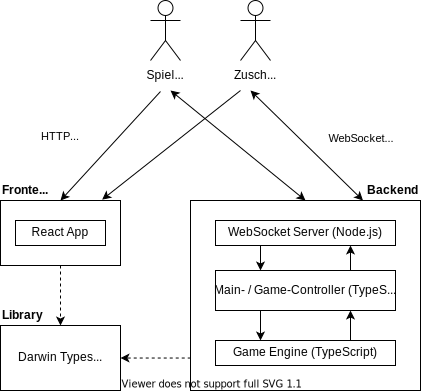
\includegraphics[width=0.9\textwidth]{architecture}
  \caption{Architektur}
\end{figure}

\subsection{Frontend}
Usability ist ein Kernanspruch an die Applikation. Deshalb verwendet Darwin moderne Technologien im Frontend.
Die Visualisierung des Spiels wird in einem 2D Canvas Context mittels Pixi.js realisiert.
Als UI-Library wird aufgrund der Erfahrung des Teams React eingesetzt.

\subsection{Backend}
Für das Backend wird Node.js eingesetzt, da dieses die meistverwendete JavaScript Runtime ist und die notwendige Stabilität aufweist.
Damit das Frontend in Echtzeit über den neusten Spielstand informiert wird, findet die Kommunikation mittels WebSockets statt.
Das Backend besteht grob beschrieben aus einem WebSocket-Server dem Main- und Game-Controller und der Game-Engine.
Der WebSocket-Server nimmt neue Verbindungen entgegen und leitet sie an die Controller weiter. Im den Controllern werden die WebSocket-Verbindungen und das Spiel als Ganzes verwaltet. Das beinhaltet auch die Verwaltung der Userskripte.
Zudem wird regelmässig ein Match-Update, welches von der Game-Engine berechnet wird, generiert und an die verbundenen Spieler und Zuschauer gesendet. 
Im Backend werden keine externen APIs verwendet und es ist insbesondere keine Persistierungsschicht angedacht.

\subsection{Darwin-Types}
Die Darwin-Types sind Typen wie zum Beispiel die Unit oder der Spielstatus, welche im Frontend sowie im Backend verwendet werden. Sie sind in einem
eigenen Node-Modul zusammengefasst, was die Nutzung von ihnen in anderen Softwareteilen enorm vereinfacht. 

\section{Code}

Der Kern des Spiels stellt die Spielelogik dar. Ziel der Logik ist es, Skripts von Benutzern sicher und fair auszuführen.
Im folgenden werden wichtige Elemente der Logik erläutert.

\subsection{Skript Ausführung}

Die Skripts werden direkt auf dem Server ausgeführt. Deshalb müssen Massnahmen für die sichere Code Ausführung ergriffen werden.
Um eine möglichst sichere Ausführung zu gewährleisten, wird eine dedizierte Bibliothek eingesetzt.
Diese ermöglicht es, für jedes Skript einen spezifischen V8 Isolate zu verwenden.

Folgende Massnahmen werden ergriffen, um häufige Missbrauchsmöglichkeiten zu verhindern:

\begin{itemize}
  \item Sowohl CPU als auch Arbeitsspeicher Limiten sind gesetzt und verhindern unzulässiges Nutzen der Ressourcen.
  \item Zugriff auf die Node.js Laufzeit des Servers ist nicht möglich.
  \item Die Skripts haben keine Möglichkeit mit dem Netzwerk, Dateisystem oder dergleichen zu kommunizieren, deshalb können sie auch nicht für Bot Netzwerke missbraucht werden.
\end{itemize}

Diese Massnahmen verkleinern den Angriffsvektor für böswillige Skripts.

\subsection{Spielelogik}

Die Befehle welche der Player absetzen kann, um das Spiel zu beeinflussen, werden als Absichten (Intents) abgebildet.
Die Gliederung der verschiedenen Intents ist in Figure \ref{fig:classDiagramIntents} ersichtlich.

\begin{figure}[h]
  \centering
  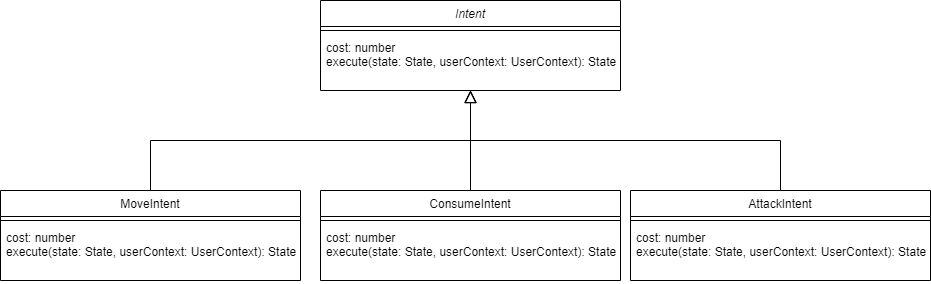
\includegraphics[width=0.9\textwidth]{Intent}
  \caption{Klassendiagramm Intents}
  \label{fig:classDiagramIntents}
\end{figure}

Die Skripts werden sequentiell ausgeführt und alle Absichten gemäss ihren Kosten pro Skript in eine künstliche Zeitachse eingegliedert.

Damit die Absichten aller Benutzer berücksichtigt werden können, wird folgender Prozess durchlaufen:
\begin{itemize}
  \item Alle individuellen Absichten in globale Ablaufreihenfolge eingliedern.
  \item Einträge innerhalb eines spezifischen Zeiteintrages zufällig anordnen. Somit wird kein Spieler bevorzugt.
  \item Absichten, welche nicht im Zeitbudget erreicht werden können, entfernen. Dies stellt sicher, dass Skripts nicht unbegrenzt viele Absichten ausführen können.
\end{itemize}

Im Anschluss werden die einzelnen Zeitachseneinträge und alle gewünschten Befehle ausgeführt und auf den Spielstand appliziert.

\section{Instrastruktur-Architektur}
\label{InfrastructureArchitecture}
% Während der grösste Teil des Guidebooks sich mit der Software selber beschäftigt, wird hier die physikalische/virtuelle Infrastruktur in welche die Software installiert und betrieben wird beschrie-ben. Folgende Fragen sollten hier behandelt werden:
% • Ist eine klare Infrastruktur Architektur vorhanden?
% • Welche Hardware (virtuell oder physikalisch) wird dazu verwendet?
% • Ist Redundanz, Failoverund Disaster-Recovery vorgesehen?
% • Ist die Skalierung der Infrastruktur bekannt?
% • Wer ist zuständig für Support und Unterhalt der Infrastruktur?
% • Wer ist verantwortlich für die Ressourcen (ownership)?•etc.

Da es sich um ein Schulprojekt handelt und sich das Projekt in der Entwicklungsphase befindet, ist die Infrastruktur zurzeit simpel gehalten. Es wurde jedoch bereits angedacht, wie die Infrastruktur in Zukunft aussehen könnte.

\subsection{Infrastruktur während der Entwicklungsphase}
Wie auf der Abbildung zu sehen, wird aktuell ein Linux Rechner (mit Ubuntu 18.04.4 LTS) eingesetzt. Auf diesem ist Docker installiert, der mittels Docker-Compose jeweils einen Docker-Container für das Frontend und einen für das Backend konfiguriert. Das Backend wird mittels eines Node.js-Images betrieben, wobei für das Frontend ein Nginx-Image verwendet wird, um die statischen Dateien des gebauten React-Apps auszuliefern.

\begin{figure}[h]
  \centering
  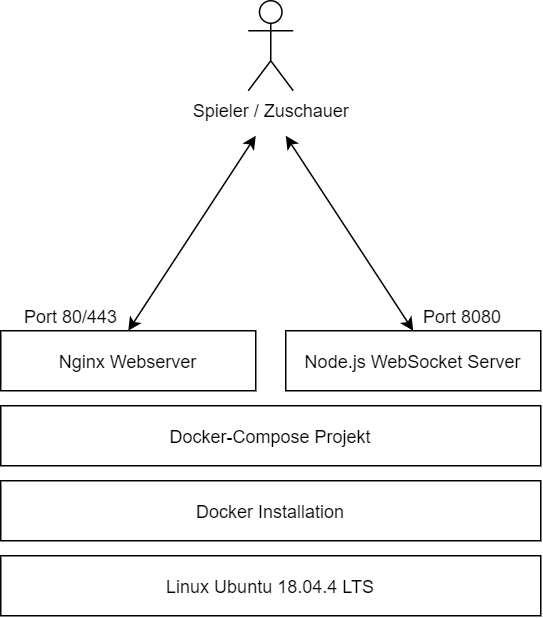
\includegraphics[width=0.5\textwidth]{infrastructure_current.png}
  \caption{Aktuelle Infrastruktur}
\end{figure}

\subsection{Skalierbarkeit und Infrastruktur in Zukunft}
Durch den Einsatz von Docker kann die Software auf einer Reihe von Systemen, wie einzelnen physikalischen/virtuellen Rechnern oder PaaS Anbietern, betrieben werden. Es besteht auch die Möglichkeit der Orchestrierung: 
\begin{itemize}
  \item Der Webserver für das Frontend, hat keinen Zustand zu speichern. Mittels eines Load Balancers kann die Last so auf mehrere Server verteilt werden.
  \item Das Backend hingegen hält den aktuellen Zustand eines Spiels und deren Spielern und Zuschauern. Daher kann man nicht während des Spiels oder in einer neuer Sitzung, während das Match noch läuft, auf einen anderen Server verbinden. Mittels eines Load Balancers, der für die verschiedenen User speichert, welcher Backend Server für den jeweiligen User zuständig ist, kann das Problem umgangen werden. Allerdings ist dies noch zu untersuchen.
\end{itemize}

Die Zuständigkeiten sind zurzeit nicht bekannt. Auch steht noch kein Konzept bezüglich Disaster-Recovery / Failover. Allerdings ist aufgrund des Einsatzes von Docker und Load Balancers bereits Vorarbeit geleistet.

% Ein Beispiel, wie eine Infrastruktur aussehen könnte:
% TODO: ? Beispielgrafik

\section{Installation (Deployment)}

Um einen raschen Release-Zyklus zu gewährleisten, wurde eine Build- sowie eine Releasepipeline eingerichtet.
Diese ermöglicht es, Pull-Requests automatisch zu testen und nach einem erfolgten Merge automatisiert zu releasen und deployen.
Dies soll die Entwicklungsphase beschleunigen und gewähleisten, dass stets und ausschliesslich funktionierender Code deployed wird.

\subsection{Build Pipeline}
Innerhalb dieser Pipeline werden folgende Schritte durchgeführt:
\begin{enumerate}
  \item Installieren aller notwendigen Pakete
  \item Linting und Formatierung werden überprüft
  \item Build wird durchgeführt
  \item Tests werden durchgeführt
  \item Bilden eines Artefakts mit Inhalt: Frontend, Backend und Shared Types
\end{enumerate}
Das Build schlägt fehl, sobald ein Schritt nicht erfolgreich war. Wenn zum Beispiel das Linting / die Formatierung nicht korrekt ist, wird das Build abgebrochen und der Pull-Request kann nicht gemerged werden.

\subsection{Release Pipeline}
Die Release Pipeline verwendet das neuste von der Build Pipeline erstellte Artefakt. Beim erfolgreichen Abschluss der Build Pipeline wird automatisch die Release Pipeline angestossen, die folgende Schritte durchführt:
\begin{enumerate}
  \item Entpacken und kopieren des Artefakts auf den Server
  \item Kopieren der Ordner aus dem Artefakt in das Docker-Compose Projekt
  \item Neuerstellen der Docker Container mittels Docker-Compose
\end{enumerate}

Wie bereits im Kapitel \textit{\nameref{InfrastructureArchitecture}} erwähnt, ist das Docker-Compose Projekt mit einem Webserver und Node.js konfiguriert.

\section{Operation und Support}

Da unser Projekt als zeitlich begrenztes Projekt einer Studenten-Gruppe läuft, ist keinerlei Support oder Maintenance nach Ablauf der Entwicklungsphase geplant.

\section{Entscheidungs-Logbuch}

\begin{itemize}
  \item 21.02.2020
        \begin{itemize}
          \item Wir haben auf das Genre "Survival" geeinigt. Dies, da es ein sehr flexibles Genre ist, mit dem bereits durch eine sehr einfache Spielmechanik (Hunger) das Grundprinzip umgesetzt werden kann.
          \item Wir haben uns entschieden, die Steuerung mittels Code zu machen, da es erst wenige Spiele mit einer solchen Steuerung gibt und uns die technischen sowie auch Gameplay-spezifischen Aspekte interessieren.
          \item Wir setzen Frontend und Backend mittels JavaScript (TypeScript) um, da unser Know-how mit dieser Sprache am höchsten ist und sie uns hohe Flexibilität bietet.
        \end{itemize}
  \item 04.03.2020
        \begin{itemize}
          \item Branches werden gelöscht, sobald sie in den Master-Branch gemerged wurden. Das ver-bessert die Übersicht im Repository. Der Pull Request bleibt bestehen, da dort nachvollzogen werden kann, wie man zu einem Entschluss gekommen ist.
          \item Beim mergen eines Pull-Requests muss die Option "Squash Commits" gewählt werden. Diese Option fasst alle Commits aus dem Branch in einen zusammen. So bleibt der Master-Branch sauber und es ist ersichtlich wann welches Feature hinzugefügt wurde.
          \item Bevor ein Pull-Request gemerged werden darf, muss mindestens eine andere Person die Änderungen durchgeschaut haben (4-Augen-Prinzip).
        \end{itemize}
  \item 11.03.2020
        \begin{itemize}
          \item Das Theme des Spiels wurde der Einfachheit halber vom Willhelm Tell auf "Geometrische Figuren" geändert.
        \end{itemize}
  \item 12.03.2020
        \begin{itemize}
          \item Ursprung des Koordinatensystems für die Berechnung der Befehle und die Darstellung des Spiels ist oben links
                mit steigenden Koordinaten nach rechts und unten. Da wir für die Darstellung des Spiels Canvas verwenden und das den
                Ursprung oben links hat, haben wir uns entschieden das so durch die ganze Applikation hinweg so zu machen.
        \end{itemize}
  \item 18.03.2020
        \begin{itemize}
          \item Wir werden ab sofort ein Bi-Daily Meeting im Slack durchführen, dadurch soll klarer werden wer an was bis wann arbeitet.
          \item Wir möchten vermehrt auf Pairprogramming und 1:1 Zuweisung von erfahrenem und neueinsteigendem Entwickler um so
                Wissensunterschiede möglichst schnell auszugleichen.
        \end{itemize}
  \item 20.03.2020
        \begin{itemize}
          \item Matchlobbies werden vorerst nicht unterstützt. Diese Funktion bringt momentan nur einen geringen Mehrwert und wird daher auf unbestimmte
                Zeit verschoben.
        \end{itemize}
  \item 01.04.2020
        \begin{itemize}
          \item Die Integrationtests werden mit Jest anstatt Cypress umgesetzt. Mit Cypress wären richtige End-to-End-Tests möglich, jedoch gab es massive Probleme technischer Natur im Zusammenhang mit Canvas. 
                Aufgrund diesen Problemen verwenden wir nun Jest um ganze Komponenten wie z.B. die komplette Game-Engine zu testen.
        \end{itemize}
\end{itemize}

\clearpage

\end{document}
